%% Lee
%% In dissertation, change 
%    section* to chapter 
%    subsection* to section
%    subsubsection* to subsection

\chapter{Results}
\label{chap-six}
\label{sec:Results}
The objectives of this work was to design a system able to accelerate ANNs in customer facing systems implemented at the edge. This means systems that are not designed
to process multiple requests of essentially the same operation.
One assumption is that these systems implement disparate ANNs performing various functions. These assumptions imply that the system is not able to take advantage of local SRAM when processing the ANN.
Another assumption is that the target systems will be space and power constrained.
Finally, this work assumes that implementing multiple disparate ANNs cannot be implemented purely with SRAM and that DRAM is required to store the ANN parameters.

To demonstrate such a system, this work targeted 3DIC technology including 3D-DRAM. This work proposes that if a system can be purely 3DIC, the system can take advantage of the benefits
of 3DIC which inlcudes reduced energy, area and additional bandwidth due to high levels of connectivity.
In addition, this work proposes that if the system is purely 3DIC, then a customized DRAM would provide a significant bandwidth boost over typical implementations using standard DRAM.
This work targeted the Tezzaron DiRAM4 3D-DRAM.

To ensure the system was purely 3DIC, the area of the system Manager and Processing Engine has to stay within the physical footprint of the DRAM.

The target technology node was 28nm. This was chosen because its the technology node employed for some recent GPUs and other ASICs such as \cite{jouppi2017datacenter}.
The design was synthesized using an available 65nm technology node and then scaled to 28nm to demonstrate fitting within the 3DIC footprint.

The primary control and datapaths of the system have been simulated in a system verilog environment. It has been synthesized using a 65nm technology node.
The design has been coded targeting a frequency of $>$\SI{500}{\mega\hertz}. Timing closure and place and route is ongoing. The system has been designed throughout to meet the timing target so minimal changes are expected to meet timing.

As mention previously \eqref{eq:averageBandwidth}, to process multiple useful sized ANNs requires a sustained bandwidth to the PE of the order of ten's of \SI[per-mode=symbol]{}{\tera\bit\per\second}.
%%%%The approximate design targets are shown in Table \ref{tab:DesignTargets}.
%%%%
%%%%\begin{table}[h]
%%%%%  \captionsetup{justification=centering, skip=-5pt}
%%%%  \captionsetup{justification=centering, skip=3pt}
%%%%  \caption{Design targets}
%%%%  \label{tab:DesignTargets}
%%%%  \centering
%%%%%  \begin{center}
%%%%    % [lr] ~ left align col 0 and right align col 1
%%%%    % e.g. 4 columns could be lccr
%%%%    \begin{tabular}{lr}
%%%%      \toprule
%%%%      Parameter         & Target \\
%%%%      \midrule
%%%%      Frequency         & $>$\SI{700}{\MHz}   \\
%%%%      Power             & \SI{\approx 80}{\W}   \\
%%%%      Bandwidth         & \SI[per-mode=symbol]{\approx 64}{\tera\bit\per\second} \\
%%%%      Overall Die Area  & \SI{175}{\mm^2} \\
%%%%      \bottomrule
%%%%    \end{tabular}
%%%%%  \end{center}
%%%%\end{table}

The Manager and PE have been place and routed as shown in figure \ref{fig:Manager and PE Die layouts}. 
Although the design is yet to close timing, the parasitics were extracted from these layouts and simulated against a group of operations. The operations simulated were based on the expected lower and upper limits of pre-synaptic fanin. These were based on layers similar to CONV2 and FC-7 from \cite{krizhevsky2012imagenet} and represent a pre-synaptic fanin of 225 and 4000 respectively.
The simulation generated an activity file which was then used by the Synopsys\textregistered ~Primetime-PX\texttrademark ~power analysis tool to obtain power and bandwidth estimates.
The DRAM accesses were captured and energy used calculated from \cite{tezzaron:diram4}. The power dissipated in the TSVs were estimated from data from \cite{Bamberg2017}.
These estimates were used to estimate power dissipation for operating frequencies of \SI{500}{\mega\hertz} and \SI{700}{\mega\hertz} which are shown in table \ref{tab:Simulation-based estimates}.

\begin{table}
%  \captionsetup{justification=centering, skip=-5pt}
  \captionsetup{justification=centering, skip=12pt}
  \caption{Simulation-based estimates}
  \vspace{12pt}
  \label{tab:Simulation-based estimates}
  \centering
    % [lr] ~ left align col 0 and right align col 1
    % e.g. 4 columns could be lccr
  \begin{subtable}{0.55\linewidth}
    \centering
    \begin{adjustbox}{width=1\linewidth}
      \begin{tabular}{cccc}
        \toprule
                            % \multicolumn{4}{c}{3D-DRAM Simulation-based estimates}   \\
                         &                       &          &                                          \\  %\cline{1-1}
            Technology   & Clock                 & Expected &  Bus                                     \\  %\cline{1-1}
                Node     & Frequency             &  Power   &  Efficiency                              \\  %\cline{1-1}
        \hline  % instead of \midrule %midrule doesnt overlap with column lines
                   28nm  & \SI{500}{\mega\hertz} &   53W    &  \SI[per-mode=symbol]{\sim 70}{\percent} \\ %\cline{2-2}
                   28nm  & \SI{700}{\mega\hertz} &   73W    &  \SI[per-mode=symbol]{\sim 70}{\percent} \\ %\cline{2-2}
        \bottomrule
      \end{tabular}
    \end{adjustbox}
    \vspace{3pt}
    \captionsetup{justification=centering, skip=10pt}
    \caption{Power Dissipation}
    \label{tab:Power Dissipation}
  \end{subtable}

  \bigskip

  \begin{subtable}{0.65\linewidth}
    \centering
    \begin{adjustbox}{width=1\linewidth}
      \begin{tabular}{cccc}
        \toprule
                            % \multicolumn{4}{c}{3D-DRAM Simulation-based estimates}   \\
                                                       & Downstream                              &                                        \multicolumn{2}{c}{Average Downstream Bandwidth}                      \\  %\cline{1-1}
                                                       & Stack                                   &                                        \multicolumn{2}{c}{At Frequency}                                      \\  %\cline{1-1}
                   Test                                & Bus Efficiency                          &       \SI{500}{\mega\hertz}                            & \SI{700}{\mega\hertz}                               \\  %\cline{1-1}
        \hline  % instead of \midrule %midrule doesnt overlap with column lines                                       
                   CONV2 \cite{krizhevsky2012imagenet} &\SI[per-mode=symbol]{\sim 65}{\percent}  & \SI[per-mode=symbol]{\sim 43}{\tera\bit\per\second}    & \SI[per-mode=symbol]{\sim 60}{\tera\bit\per\second} \\ %\cline{2-2}
                   CONV-294                            &\SI[per-mode=symbol]{\sim 67}{\percent}  & \SI[per-mode=symbol]{\sim 44}{\tera\bit\per\second}    & \SI[per-mode=symbol]{\sim 61}{\tera\bit\per\second} \\ %\cline{2-2}
                   CONV-300                            &\SI[per-mode=symbol]{\sim 73}{\percent}  & \SI[per-mode=symbol]{\sim 48}{\tera\bit\per\second}    & \SI[per-mode=symbol]{\sim 67}{\tera\bit\per\second} \\ %\cline{2-2}
                   CONV-500                            &\SI[per-mode=symbol]{\sim 82}{\percent}  & \SI[per-mode=symbol]{\sim 54}{\tera\bit\per\second}    & \SI[per-mode=symbol]{\sim 75}{\tera\bit\per\second} \\ %\cline{2-2}
                   CONV-1000                           &\SI[per-mode=symbol]{\sim 89}{\percent}  & \SI[per-mode=symbol]{\sim 58}{\tera\bit\per\second}    & \SI[per-mode=symbol]{\sim 82}{\tera\bit\per\second} \\ %\cline{2-2}
                   FC-350                              &\SI[per-mode=symbol]{\sim 78}{\percent}  & \SI[per-mode=symbol]{\sim 51}{\tera\bit\per\second}    & \SI[per-mode=symbol]{\sim 72}{\tera\bit\per\second} \\ %\cline{2-2}
                   FC-500                              &\SI[per-mode=symbol]{\sim 84}{\percent}  & \SI[per-mode=symbol]{\sim 55}{\tera\bit\per\second}    & \SI[per-mode=symbol]{\sim 77}{\tera\bit\per\second} \\ %\cline{2-2}
                   FC-1000                             &\SI[per-mode=symbol]{\sim 91}{\percent}  & \SI[per-mode=symbol]{\sim 60}{\tera\bit\per\second}    & \SI[per-mode=symbol]{\sim 83}{\tera\bit\per\second} \\ %\cline{2-2}
                   FC-7 \cite{krizhevsky2012imagenet}  &\SI[per-mode=symbol]{\sim 94}{\percent}  & \SI[per-mode=symbol]{\sim 62}{\tera\bit\per\second}    & \SI[per-mode=symbol]{\sim 86}{\tera\bit\per\second} \\ %\cline{2-2}
        \bottomrule
      \end{tabular}
    \end{adjustbox}
    \vspace{3pt}
    \captionsetup{justification=centering, skip=10pt}
    \caption{Bus Efficiency}
    \label{tab:Bus Efficiency}
  \end{subtable}
  \end{table}


%%%%\begin{table}[h]
%%%%%  \captionsetup{justification=centering, skip=-5pt}
%%%%  \captionsetup{justification=centering, skip=3pt}
%%%%  \caption{Design targets}
%%%%  \label{tab:DesignTargets}
%%%%  \centering
%%%%%  \begin{center}
%%%%    % [lr] ~ left align col 0 and right align col 1
%%%%    % e.g. 4 columns could be lccr
%%%%    \begin{tabular}{lccccc}
%%%%          \toprule
%%%%                            %& \multicolumn{4}{c}{Technology}   \\
%%%%                            &       &       &  Usable    &          &  \\  %\cline{1-1}
%%%%                            &       &       &   DRAM     & Expected &  \\  %\cline{1-1}
%%%%                            & Tech  & Freq  & Bandwidth  &  Power   &  \\  %\cline{1-1}
%%%%          \hline  % instead of \midrule %midrule doesnt overlap with column lines
%%%%                  3D-System & 28    & \SI{700}{\mega\hertz}      &       \SI[per-mode=symbol]{\sim 64}{\tera\bit\per\second}   &  73W   &  \\ %\cline{2-2}
%%%%                  NVidia    & 28    &       &  $\ll$\SI[per-mode=symbol]{1.28}{\tera\bit\per\second} &  100W  &  \\
%%%%                  TPU       & 28    &       &  $<$  \SI[per-mode=symbol]{224}{\giga\bit\per\second}  &  40W   &  \\
%%%%          \bottomrule
%%%%    \end{tabular}
%%%%%  \end{center}
%%%%\end{table}



\begin{figure}[h]
\centering
\begin{subfigure}{.5\textwidth}
  \centering
  \centerline{
    \mbox{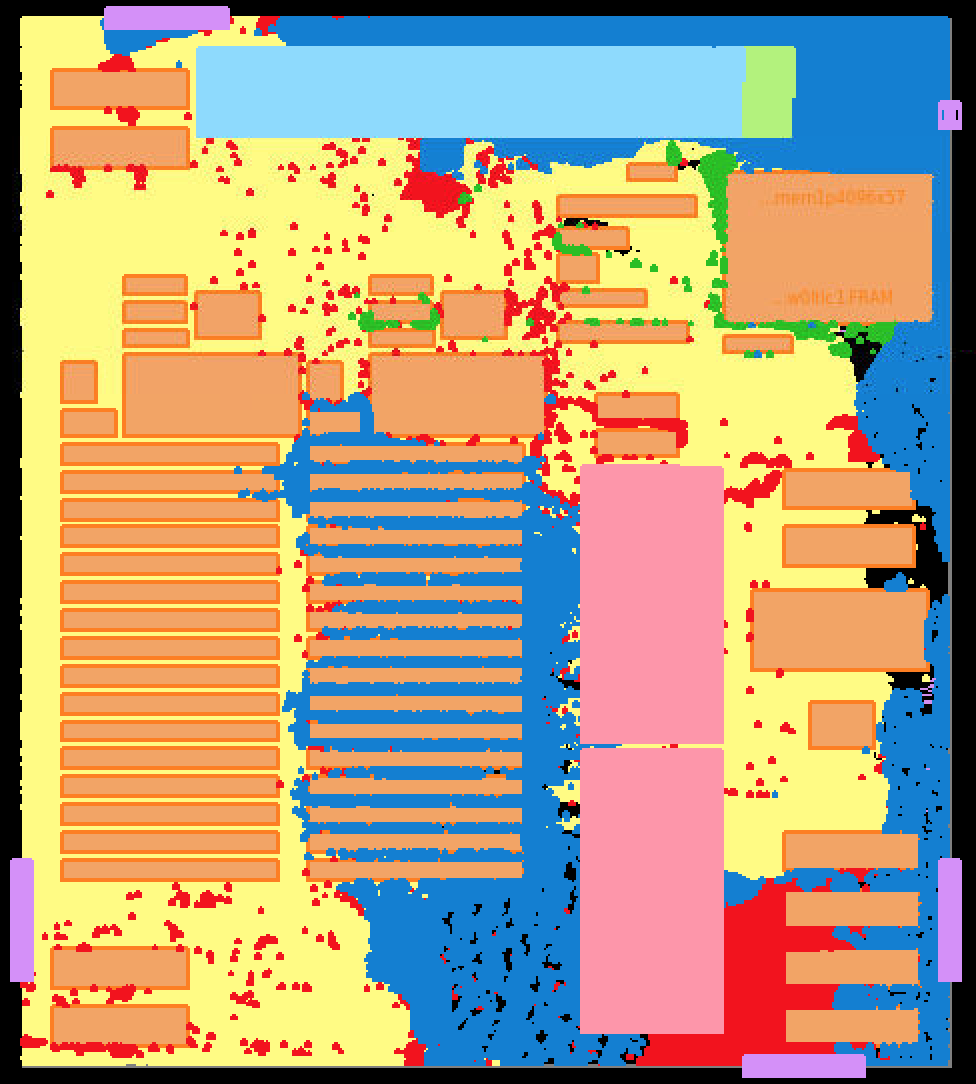
\includegraphics[width=1\linewidth]{ManagerLayout.png}}
  }
  \captionsetup{justification=centering, width=.8\linewidth}
  \caption{Manager}
  %\vspace{40pt}
  \label{fig:managerLayout}
\end{subfigure}%

\bigskip

\begin{subfigure}{.5\textwidth}
  \centering
  \centerline{
    \mbox{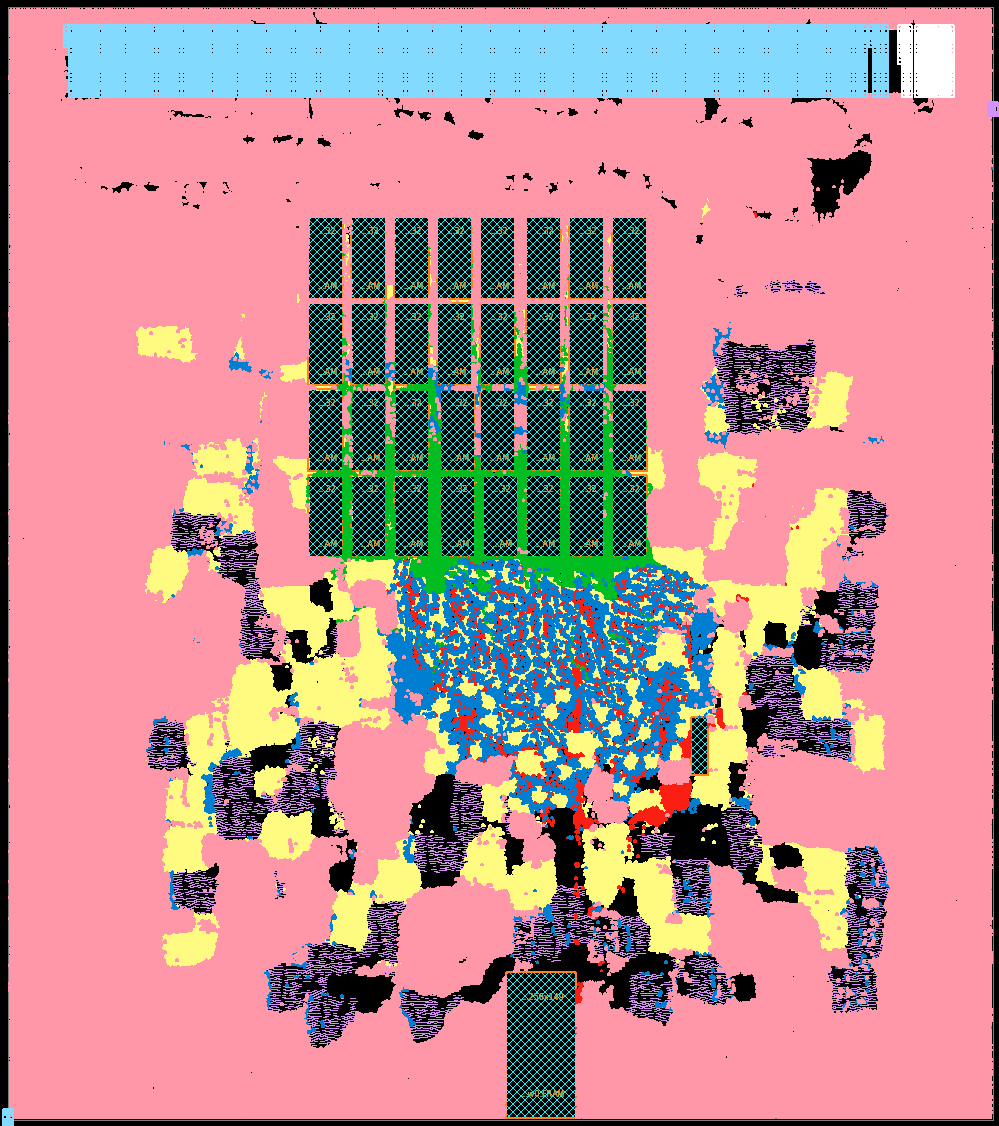
\includegraphics[width=1\linewidth]{PElayout.png}}
  }
  \captionsetup{justification=centering, width=.8\linewidth}
  \caption{PE}
  \label{fig:peLayout}
\end{subfigure}
\captionsetup{justification=centering, width=.9\linewidth}
\caption{Manager and PE Die layouts}
\label{fig:Manager and PE Die layouts}
\end{figure}


